\chapter{SEMI-STABLE LATTICE IN HIGHER RANK}
In this chapter, we will establish the notion of semi-stable lattice. Heuristically,
this is a lattice that achieve all its successive minima at the same time, see \cite{MR2153282}.

We will provide two different definitions of semi -stable lattices; one is geometric - which follows Grayson's notion of a canonical plot in \cite{MR780079}, and one is purely algebraic, which makes use of the maximal standard parabolic subgroups. We will show that the two definitions coincide in the next chapter.
\section{Lattices in higher rank}
Since lattices is the central object for studying in this thesis, we will define the notion of lattice of rank at least 3 in the last section in chapter I.
The definitions and properties of a general lattice will be used extensively in the later part of this thesis. Note that, in many reference, such as
\cite{MR780079}, the lattice is defined to be a module over a ring of algebraic integers, but we can always restrict to a $\mathbb{Z}$-module.
\subsection{Abstract lattices}
The following definition is due to \cite[section 4]{MR1905312}
\begin{definition}[\label = Abstract $\mathbb{Z}$-lattices]
    Let $L$ be a finitely generated $\mathbb{Z}$-module. In particular, it is a free $\mathbb{Z}$-module
    of finite rank. Suppose that $L$ is endowed with a map $Q\colon L \to \mathbb{R}$, such that
    the following conditions hold
    \begin{enumerate}
        \item The set $\left\lbrace x \in L: Q(x) \le r\right\rbrace $ is finite for any real number $r$ - \textbf{the parallelogram law}\label{parallelogram law}.
        \item $Q(x+y)+Q(x-y) = 2Q(x)+2Q(y)$ for all $x,y \in L$.
        \item $Q(x) \ne 0$ for all $x \in L \setminus \{0\}$.
    \end{enumerate}
    We will call  the pair $(L,Q)$ a \textbf{abstract $\mathbb{Z}$-lattice}.
\end{definition}

\begin{example}\label{standard-lattice-zn}
    Take $L = \mathbb{Z}^n$ and choose our quadratic form to be the standard one. In particular, for $x = (x_1,x_2,\ldots,x_n) \in \mathbb{Z}^n$,
    \[Q(x):= x_1^2+x_2^2+\ldots +x_n^2\]
    Here the multiplication is just the usual dot product between 2 vectors. In term of matrix, this quadratic form is assigned to the
    identity matrix $I_n$.
\end{example}
If there is no further confusion, we can just denote a Euclidean lattice by $L$, without specifying the bilinear form
$Q$. The lattice $L$ determines a full-rank lattice inside $L_\mathbb{R}$, namely, the rank
of the lattice $L$ is equal to the dimension of $L_\mathbb{R}$.

\subsection{An alternative definition of lattices}
For the sake of computation, we also usually adopt another definition of the lattice.
In particular, we view lattice as a free $\mathbb{Z}-$ module of rank $n$ that is isomorphic
to $\mathbb{R}^n$ via base changing.
\begin{definition}\label{lattice2}
    A \textit{lattice} in $\mathbb{R}^n$ is a subset $L \subset \mathbb{R}^n$ such that there exists
    a basis $b_1,\ldots,b_n$ of $\mathbb{R}^n$ such that
    \[L = \mathbb{Z}b_1\oplus \mathbb{Z}b_2\oplus \ldots \mathbb{Z}b_n\]
    If we put the vector $b_1,b_2,\ldots,b_n$ in columns, with respect to the standard basis, namely
    \[g = [b_1 | b_2 | \ldots | b_n] ,\]
    then $L = g\mathbb{Z}^n$.
\end{definition}
It can be shown that $L$ is a discrete subset of $\mathbb{R}^n$ . The discrete property turns out to be the sufficient condition for a subset of $\mathbb{R}^n$ to be a lattice, as stated in the
following proposition
\begin{theorem}\cite[Proposition 4.2]{MR1697859}\label{discrete-lattice}
    Given a vector space $V$ and a subset $L \subset V$. Then $L$ is a lattice if and only if $L$ is discrete.
\end{theorem}

\subsection{Equivalence between two definitions of lattices}
In this subsection, we will show that every abstract $\mathbb{Z}$- lattice is isomorphic to an Euclidean $\mathbb{Z}-$ lattice.
This will be helpful in visualizing the abstract lattices, as we are just looking at concrete lattices with deformation by a linear transformation.
First we need to specify the notion of isomorphic lattices - in the first definition
\begin{definition}
    A map $f \colon (L,Q)   \to (L',Q')$  is an \textbf{isomorphism} between lattices if it is a group isomorphism and
    for all $x \in L$, we have
    \[Q(x) = Q'(f(x)) \]
\end{definition}
\begin{prop}\label{equiv-def}
    Any abstract lattice is isomorphic to a Euclidean $\mathbb{Z}-$ lattice.
\end{prop}
\begin{proof}
    Assume that $L=\mathbb{Z}b_1\oplus \mathbb{Z}b_2\oplus \ldots \mathbb{Z}b_n$, and choose the associated quadratic form as in example \ref{standard-lattice-zn}, we can directly
    verify that the 3 conditions defining an abstract lattice hold. Conversely, we define
    \[\left\langle x,y\right\rangle:=\dfrac{Q(x+y)-Q(x-y)}{4}\]
    We will show that this can be extended to an inner product on $\mathbb{R}^n = L \otimes \mathbb{R}$. By the parallelogram law \ref{parallelogram law}, we have $Q(y-x) = 2Q(x)+2Q(y)-Q(x+y) = Q(x-y)$, thus
    \[\left\langle x,y \right\rangle=\dfrac{Q(x+y)-Q(x-y)}{4} = \dfrac{Q(x+y)-Q(y-x)}{4} = \left\langle y,x \right\rangle\]
    We will prove by induction that $Q(mx) = m^2Q(x)$ for all positive integer $m$. The statement is trivial for $m=1$. By parallelogram law
    \[Q(mx) = 2Q[(m-1)x] + 2Q(x) - Q[(m-2)x] = [2(m-1)^2+2-(m-2)^2]Q(x) = m^2Q(x)\]
    As a consequence, $Q(x) \ge 0$ for all $x \in L$. Indeed, if $Q(x)<0$ for some $x \in L$, then the set $\{v \in L: Q(v)<0\}\supset \mathbb{Z}x$, hence infinite. But this contradicts
    the condition 3 of an abstract lattice. Finally, consider the relations
    \begin{align*}
        Q(a+b+c) +Q(a-b+c) = 2Q(a+c)+2Q(b) \\
        Q(a+b-c)+ Q(a-b-c) = 2Q(a-c)+2Q(b) \\
        Q(a+b+c)+ Q(a-b-c) =2Q(b+c)+2Q(a)  \\
        Q(a+b-c)+ Q(a-b+c) =2Q(b-c)+2Q(a)
    \end{align*}
    Taking the alternative sum yields
    \[2Q(a+b+c)-2Q(a+b-c) = 2Q(a+c)-2Q(a-c) + 2Q(b+c)-2Q(b-c) \]
    or equivalently
    \[\left\langle a+b,c\right\rangle = \left\langle a,c\right\rangle+ \left\langle b,c\right\rangle \]
    Thus we can extend  the function $\left\langle \cdot,\cdot \right\rangle \colon L \times L\to \mathbb{R}$ to a $\mathbb{R}$-bilinear function over $L_\mathbb{R} \times L_\mathbb{R}$ by
    taking the tensor product. Clearly $Q(x/m) = \dfrac{1}{m^2}Q(x)$ for any $m \in \mathbb{Z} \setminus \{0\}$ and $x\in L$. Moreover the set $\{x/m: x \in L, m \in \mathbb{Z} \setminus \{0\}\}$ is dense
    in $L_\mathbb{R}$, hence $Q$ define a norm on $L_\mathbb{R}$. In particular, $\left\langle \cdot, \cdot\right\rangle$ extends to an inner product on $L_\mathbb{R}$. The discrete condition of the abstract lattice ensure that
    $L$ is a discrete subset of $L_\mathbb{R}$ hence an Euclidean lattice by theorem \ref{discrete-lattice}.
\end{proof}
\subsection{Covolume of a lattice}
Now that for every abstract lattice $L$ we can find an invertible matrix $g$ such that
\[ L  \cong g\mathbb{Z}^n\]

The number $n$ is called the \textbf{rank} of the lattice $L$.

Let $\left\lbrace e_1,e_2,\ldots,e_n \right\rbrace$ be an orthonormal basis of $L_\mathbb{R} \cong \mathbb{R}^n$ and
\[g = [b_1 | b_2 | \ldots | b_n] .\] The covolume of the lattice
$L$ is defined as
\begin{definition}\label{covolume-lattice-formula}
    The covolume of $L$ is given by the formula
    \[\vol(L) = \left|\det(\left\langle b_i,e_j\right\rangle)\right|\]
\end{definition}
The rank and covolume are invariant numerical values of $L$, as they don't depend on the choice of basis. Indeed, two bases of a rank $n$ lattice $L$
are related by a transformation $g \in \text{GL}_n(\mathbb{Z})$. Clearly this preserves the volume and the rank as a $\mathbb{Z}-$module.


\subsection{Sublattices}
To work with semi-stable lattice $L$, we need to consider all the sublattices contained inside $L$.
\begin{definition}[\label=sublattice]
    Let $(L,Q)$ be a Euclidean $\mathbb{Z}$-lattice. We say that a $\mathbb{Z}-$submodule $M$ of
    $L$ a \textbf{sublattice} if and only if $L/M$ is torsion free.
\end{definition}
From this definition, we can prove that $M$ is a sublattice of $L$ if it satisfies one of the
following equivalent properties:
\begin{enumerate}
    \item $M$ is a summand of $L$.
    \item every basis of $M$ can be extended to a basis of $L$.
    \item The group $M$ is an intersection of $L$ with a rational subspace of $L_\mathbb{R}$.
\end{enumerate}
We refer to the \cite[Section 1.4]{MR4505757} for a proof of these equivalences.
\begin{example}
    If $L = \mathbb{Z}^2$, then any sublattice of $L$ is a primitive vector $u = (a,b)$, i.e
    $\gcd(a,b)=1$. Indeed, $u=(a,b)$ is a sublattice of $\mathbb{Z}^2$ if and only if there exists a vector $v \in \mathbb{Z}^2$
    such that $L = \mathbb{Z}u \oplus \mathbb{Z}v$. With respect to the usual inner product on $\mathbb{R}^2$,
    we have
    \[1 = \vol(\mathbb{Z}^2) = \det \begin{bmatrix}
            a & b \\
            c & d
        \end{bmatrix} = ad-bc\]
    This happens if and only if $\gcd(a,b)=1$.
\end{example}

\begin{definition}
    Given a lattice $L$ and a subgroup $M \subset L$, then we call the  $M$ \textbf{primitive } if $L/M$ is torsion free. Equivalently, $M \subset L $ is a
    primitive sublattice if no non-zero multiples of non-members of $M$ are in M. In formula
    \[(M \otimes \mathbb{Q}) \cap L = M\]
\end{definition}
\begin{example}
    We consider the subgroup $M$ generated by a single element $v \in L$. Then $\mathbb{Z}v$ is primitive if and only if there is no $w \in L \setminus \{v\}$ such that
    \[w = c\cdot v,\]
    for some integer $c$.
\end{example}
\subsection{Exterior product and covolume of lattice}
In certain situation, it is more convenient to work with exterior product of lattices. We briefly recap the related definitions and
results here. Further information can be found in \cite[Chapter 5]{MR504976}.
\begin{definition}
    Given a vector space $V$. Then the exterior power $\bigwedge^r V$ is defined to be the vector space spanned by element
    of the form \[v_1 \wedge v_2 \wedge \ldots \wedge v_r, \quad v_i \in V\]
    subjected to the following relations
    \begin{enumerate}
        \item $v \wedge v = 0$ for all $v \in V$.
        \item $v \wedge w = -w \wedge v$ for any $v,w \in V$.
        \item $(av_1+bv_2)\wedge w = a(v_1 \wedge w)+b(v_2 \wedge w)$ for any $v_1,v_2,w \in V$.
    \end{enumerate}
\end{definition}
If we identify $V \cong \mathbb{R}^n$, then the action of $g \in \mathrm{GL}_n(\mathbb{R})$ on $\mathbb{R}^n$ via matrix multiplication $gv$ can be extended
to $\bigwedge^r V$ by defining
\[g(v_1\wedge \ldots \wedge v_r):=(gv_1 \wedge \ldots \wedge gv_r),  \quad\forall v_i \in V\]
Given an inner product $\left\langle \cdot,\cdot \right\rangle$ on $V$, the vector space $\bigwedge^r V$ also has an inner product as stated in the following theorem
\begin{theorem}\label{wedge-inner-prod}\cite[Section 5.6]{MR504976}
    There is an inner product on $\bigwedge^r V$ induced by the inner product $\left\langle \cdot,\cdot \right\rangle$ on $V$ given by
    \[\left\langle v_1 \wedge \ldots \wedge v_r, w_1 \wedge \ldots \wedge w_r \right\rangle = \det
    \begin{bmatrix}
    \left\langle v_1,w_1\right\rangle      &    \left\langle v_2,w_1\right\rangle    & \ldots & \left\langle v_r,w_1\right\rangle             \\
     \left\langle v_1,w_2\right\rangle      &    \left\langle v_2,w_2\right\rangle    & \ldots & \left\langle v_r,w_2\right\rangle             \\
     \vdots & \vdots & \ddots & \vdots\\
      \left\langle v_1,w_r\right\rangle      &    \left\langle v_2,w_r\right\rangle    & \ldots & \left\langle v_r,w_r\right\rangle             \\
    \end{bmatrix}\]
\end{theorem}
From the above theorem we can define the norm on $\bigwedge^r V$ to be 
\begin{equation}\label{wedge-norm}
    |v_1\wedge \ldots \wedge v_r| := \sqrt{\left\langle v_1\wedge \ldots \wedge v_r,v_1\wedge \ldots \wedge v_r\right\rangle}
\end{equation}
From the equation \eqref{wedge-norm}, we can derive the following result
\begin{lemma}
    Let $L$ be a lattice of rank $n$ and $\{v_1,\ldots,v_n\}$ be a basis for $L$. Then 
    \[|v_1\wedge \ldots \wedge v_n| = \vol(L)\]
\end{lemma}
\begin{proof}
    Let $\{e_1,\ldots,e_n\}$ be an orthonormal basis of the vector space $L_\mathbb{R} = L \otimes \mathbb{R}$. By definition \ref{volume-of-lattice}, we have 
    \[\vol(L) = \left\langle v_1\wedge \ldots \wedge v_n, e_1\wedge \ldots \wedge e_n\right\rangle\]
    On the other hand, the space $\bigwedge^n L_\mathbb{R}$ has dimension one, so there exists $c \in \mathbb{R}$ such that 
    \[v_1\wedge v_2 \wedge \ldots \wedge v_n = c e_1 \wedge e_2 \wedge \ldots \wedge e_n\]
    Let $v = v_1\wedge v_2 \wedge \ldots \wedge v_n$ and $e = e_1 \wedge e_2 \wedge \ldots \wedge e_n$, then we have 
    \begin{align*}
        |c|\vol(L)  =|c| \left\langle v,e \right\rangle
                    =c^2\left\langle e,e\right\rangle 
                    =c^2
    \end{align*}
    which implies that $|c| = \vol(L)$. On the other hand $\left\langle v,v\right\rangle = c^2 \left\langle e,e\right\rangle =c^2$, thus we are done proving $|v_1\wedge \ldots \wedge v_n| = \vol(L) $. \qedhere
 
\end{proof}
\section{Grayson's definition of semi-stability}
Recall that a lattice is a pair $(L,\left\langle\cdot,\cdot\right\rangle)$ where $L$ is a $\mathbb{Z}$-module
and $\left\langle\cdot,\cdot\right\rangle$ is the associated inner product. If there is no confusion, we can will just denote this lattice by $L$ - the underlying $\mathbb{Z}$-module, and $\left\langle \cdot,\cdot\right\rangle$ for  the associated inner product.
\subsection{Grayson's definition}
In this subsection, we introduce Grayson's definition of \textit{semi-stable} lattices, follows \cite{MR780079}.
Grayson associates to every lattice a convex hull of certain points in $\mathbb{R}^2$ - called its \textit{ profile}.
To define the profile, observe first that if $M \subset L$ is a sublattice, then the space $M_\mathbb{R} = M \otimes \mathbb{R}$
is a subspace of $L_\mathbb{R}$, equipped with the restriction of the positive definite symmetric form $Q$ of $L$, then $M$
is also a lattice of rank not exceeding rank of $L$.
\begin{definition}[\label = slope]
    The slope of a non-zero lattice $L$ is the number
    \[\mu(L) = \dfrac{\log\vol(L)}{\dim L}\]
\end{definition}
\begin{definition}
    Consider a lattice $L$. For any sublattice $M \subset L$, define
    \[\ell(M) = \left(\dim M, \log\vol(M)\right) \in \mathbb{R}^2.\]
    The collection of all points $\ell(M)$ where $M$ ranges over
    all sublattices of $L$ is called \textbf{ the canonical plot} of the lattice $L$. By convention, we assign
    the lattice of zero rank to the origin of the plane.
\end{definition}


The following lemma asserts that, on each vertical line $x =n$ where $(n=0,1,\ldots, \text{rk}(L))$, there is a lowest point and so the canonical plot is bounded below.
\begin{lemma}
    Given a lattice $L$ and a number $c$, there exists only a finite number of sublattices $M \subset L$ such that
    $\vol(M)<c$.
\end{lemma}
\begin{proof}
    We will prove this by induction on the rank of the sublattices.
    \begin{itemize}
        \item For $r =1$, the collection of all rank $1$ sublattices of $L$ is just the set of all vectors in $L$. So we reduce
              to show that for any $c>0$, the set $B(0,c) \cap L$  has finitely many elements. But the lattice $L$ is a discrete subset of $L_\mathbb{R}$, thus the intersection of $L$ with a bounded set has only finitely many elements.
        \item Let $r>1$. Consider
              \[M = \mathbb{Z}m_1\oplus \ldots \oplus\mathbb{Z}m_r\]
              The wedge product $\bigwedge^r L$, then clearly
              $m_1\wedge m_2\ldots \wedge m_r$ is a vector in the lattice  $\bigwedge^r L$.
              By the previous case, there are finitely
              many vectors with bounded length inside lattice. So we only need to show that the map
              \[ M \mapsto \bigwedge^r M \]
              is finite to one, then we are done. Indeed, let $v= \bigwedge^r M$ be a vector in $\bigwedge^r L$. We want to show that there are only finitely many sublattices $N \subset L$  of rank $r$  such that
              $\bigwedge^r N = v$. Indeed, let $\{n_1,n_2,\ldots n_r\}$ be a basis for $N$ then
              \[v = m_1\wedge m_2\ldots \wedge m_r = n_1\wedge n_2\ldots \wedge n_r \Rightarrow M \otimes \mathbb{Q} = N \otimes \mathbb{Q}\]
              If this is not true, we would find a factor $u \in \mathrm{span}_\mathbb{Q}(n_1,\ldots,n_r) - \mathrm{span}_\mathbb{Q}(m_1,\ldots,m_r)$. But this implies
              \[0 = u\wedge n_1 \wedge\ldots \wedge n_r = u \wedge m_1 \wedge \ldots \wedge m_r \ne 0\]
              which is a contradiction. Furthermore, we note that $N$ and $M'$ are lattice of $L$ with the same rank, so $N$ must have finite index in $M'$. This index is the same as index of $M$ in $M'$.
              In particular, the preimage of the map $M \mapsto \bigwedge^r M$ must be a abelian subgroup of $M'$ with fixed index.  There are finitely many such group, by
              \cite[Proposition A.1]{MR1460018}. Hence we are done. \qedhere
    \end{itemize}
\end{proof}
\begin{definition}
    The boundary polygon of the convex hull of the canonical plot is called \textbf{profile} of the lattice $L$.
\end{definition}
In theory, we can compute the profile by searching for the shortest vector in each of its exterior product, but this computation
is infeasible when the dimension of the lattice grows. Since there are lattices with
arbitrarily large volume of any rank smaller than that of $L$, we add to the side the point $(0,\infty)$ and $(n,\infty)$. The sides
of the profile are therefore two vertical lines. The bottom is a convex polygonal consisting of consecutive lines connecting the origin with the point $\ell(L)$.
\begin{definition}\label{ss1}
    If the bottom of the profile contains only two points $(0,0)$ and $(n,\log\vol L)$, then the
    lattice $L$ is said to be \textbf{semi-stable}. Otherwise $L$ is said to be \textbf{unstable}.
\end{definition}
Below are the picture of two lattices.
\begin{figure}[hbt]
    \centering
    \begin{minipage}{.2\textwidth}
        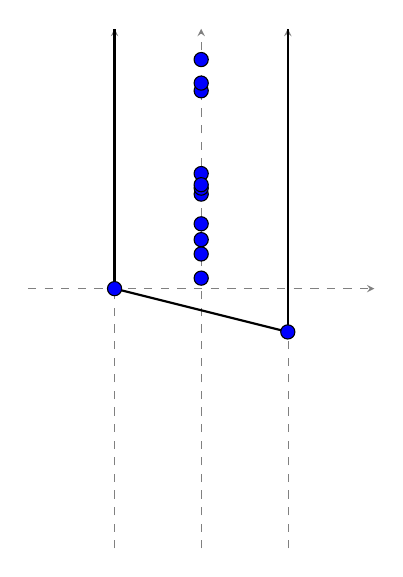
\begin{tikzpicture}[>=stealth, x=1.1cm, y=1.1cm]
            % Dashed lines (axes)
            \draw[help lines, dashed, ->] (-1,0) -- (3,0);
            \draw[help lines, dashed, ->] (0,-3) -- (0,3);
            \draw[help lines, dashed, ->] (1,-3) -- (1,3);
            \draw[help lines, dashed, ->] (2,-3) -- (2,3);
            \draw[thick] (0,0) -- (0,3);
            \draw[thick] (0,0) -- (2, -0.5);
            \draw[thick]  (2,-0.5) -- (2,3);
            \draw[thick]  (2,-0.5) -- (2,3);

            % Points (all with fill=blue and radius=0.09cm)
            \filldraw[fill=blue] (2, -0.5) circle[radius=0.09cm];
            \filldraw[fill=blue] (0, 0) circle[radius=0.09cm]; % Removed duplicate
            \filldraw[fill=blue] (1, 0.12122108098130914) circle[radius=0.09cm];
            \filldraw[fill=blue] (1, 2.28412917072110916) circle[radius=0.09cm];
            \filldraw[fill=blue] (1, 2.3729881287610001) circle[radius=0.09cm];
            \filldraw[fill=blue] (1, 0.4) circle[radius=0.09cm];
            \filldraw[fill=blue] (1, 0.5655158711807637) circle[radius=0.09cm];
            \filldraw[fill=blue] (1, 2.6445016116606668) circle[radius=0.09cm];
            \filldraw[fill=blue] (1, 0.7481703960405396) circle[radius=0.09cm];
            \filldraw[fill=blue] (1, 1.3282219276898275) circle[radius=0.09cm];
            \filldraw[fill=blue] (1, 1.0912647062501184) circle[radius=0.09cm];
            \filldraw[fill=blue] (1, 1.1603772291700336) circle[radius=0.09cm];
            \filldraw[fill=blue] (1, 1.2) circle[radius=0.09cm];
        \end{tikzpicture}~ \caption{A semi-stable lattice}
    \end{minipage} \hspace{3cm} \begin{minipage}{.2\textwidth}
        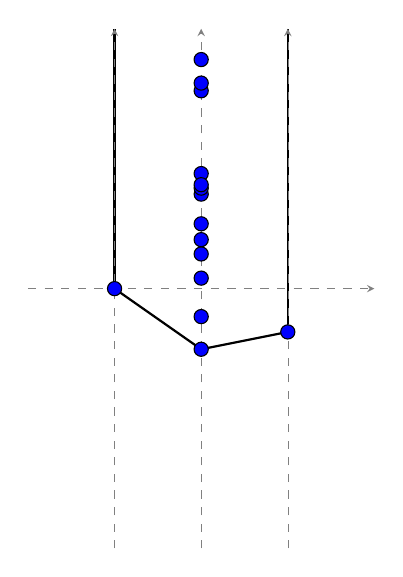
\begin{tikzpicture}[>=stealth, x=1.1cm, y=1.1cm]
            % Dashed lines (axes)
            \draw[help lines, dashed, ->] (-1,0) -- (3,0);
            \draw[thick] (0,0) -- (0,3);
            \draw[thick] (0,0) -- (1, -0.7);
            \draw[thick] (1,-0.7) -- (2,-0.5);
            \draw[thick]  (2,-0.5) -- (2,3);
            \draw[help lines, dashed, ->] (0,-3) -- (0,3);
            \draw[help lines, dashed, ->] (1,-3) -- (1,3);
            \draw[help lines, dashed, ->] (2,-3) -- (2,3);

            % Points (all with fill=blue and radius=0.09cm)
            \filldraw[fill=blue] (2, -0.5) circle[radius=0.09cm];
            \filldraw[fill=blue] (0, 0) circle[radius=0.09cm]; % Removed duplicate
            \filldraw[fill=blue] (1, -0.7) circle[radius=0.09cm];
            \filldraw[fill=blue] (1, -0.3230737092181455) circle[radius=0.09cm];
            \filldraw[fill=blue] (1, 0.12122108098130914) circle[radius=0.09cm];
            \filldraw[fill=blue] (1, 2.28412917072110916) circle[radius=0.09cm];
            \filldraw[fill=blue] (1, 2.3729881287610001) circle[radius=0.09cm];
            \filldraw[fill=blue] (1, 0.4) circle[radius=0.09cm];
            \filldraw[fill=blue] (1, 0.5655158711807637) circle[radius=0.09cm];
            \filldraw[fill=blue] (1, 2.6445016116606668) circle[radius=0.09cm];
            \filldraw[fill=blue] (1, 0.7481703960405396) circle[radius=0.09cm];
            \filldraw[fill=blue] (1, 1.3282219276898275) circle[radius=0.09cm];
            \filldraw[fill=blue] (1, 1.0912647062501184) circle[radius=0.09cm];
            \filldraw[fill=blue] (1, 1.1603772291700336) circle[radius=0.09cm];
            \filldraw[fill=blue] (1, 1.2) circle[radius=0.09cm];
        \end{tikzpicture}~
        \caption{An unstable lattice}
    \end{minipage}
\end{figure}
Visually, a lattice is called \textbf{semi-stable} if it satisfies the other equivalent
conditions:   If $M$ is an arbitrary sublattice of $L$ then $\mu(M) \ge \mu(L)$.
\subsection{Canonical filtration}
Given a lattice $L$ and a sublattice $M \subset L$, the quotient group $L/M$ has the structure of
a lattice. Indeed, consider the exact sequence of lattices
\[0\rightarrow M\rightarrow L\rightarrow L/M\rightarrow 0\]
By tensoring with $\mathbb{R}$ we get a short exact sequence of $\mathbb{R}$-vector subspaces
\[0\rightarrow M_\mathbb{R} \rightarrow L_\mathbb{R} \rightarrow (L/M)_\mathbb{R}\rightarrow 0,\]
which is split. Thus we have the isomorphisms
\[(L/M)_\mathbb{R} \cong L_\mathbb{R}/M_\mathbb{R} \cong M^\perp_\mathbb{R}\]
Therefore, by restricting of the inner product over $L_\mathbb{R}$ to $M^\perp_\mathbb{R}$, we clearly see that
$L/M$ also inherits an inner product. Explicitly, the norm over $L/M$ can be defined by restricting the norm $||\cdot||$ on $L_\mathbb{R}/M_\mathbb{R}$, which is given by
\[||x||:= \inf\{ ||x+m||: m \in M \}\]
\begin{definition}
    Given a lattice $L$ containing a sublattice $M$, then $L/M$ is a lattice. We call this lattice \textbf{quotient lattice}.
\end{definition}
\begin{lemma}\label{volume-of-lattice}\cite[Proposition 4.1]{MR2127941}
    If $L$ is a lattice and $M\subset L$ is a sublattice, we have
    \[\vol(L) = \vol(M)\cdot \vol(L/M)\]
    and if $N$ is any sublattice of $L$ that satisfies $N+M=L$ then
    \[\vol(N) \ge \vol(L/M)\]
\end{lemma}
\begin{proof}
    Assume that $\{m_i\}$ is a basis for the lattice $M$ and $\{e_i\}$ be an orthonormal basis for the vector space
    $M_\mathbb{R}$. Since $M$ is a sublattice of $L$, we can extend the basis $\{m_i\}$ to get a
    basis $\{m_i\} \cup \{n_j\}$ for the lattice $L$. Similarly, we can extend  $\{e_i\}$ to get an orthonormal
    basis $\{e_i\} \cup \{f_j\}$ for the vector space $L_\mathbb{R}$. In particular, we would have
    $\left\langle m_i,f_j \right\rangle =0$ for all $i,j$.
    By definition \ref{covolume-lattice-formula}, we have
    \begin{align*}
        \vol(L) & = \det\begin{bmatrix}
                            \left\langle m_i,e_i\right\rangle  & \left\langle n_j,e_i\right\rangle \\
                            \left\langle m_i,f_J \right\rangle & \left\langle n_j,f_j\right\rangle
                        \end{bmatrix} \\
                & = \det\begin{bmatrix}
                            \left\langle m_i,e_i\right\rangle & \left\langle n_j,e_i\right\rangle \\
                            0                                 & \left\langle n_j,f_j\right\rangle
                        \end{bmatrix}  \\
                & =\vol(M)\cdot \vol(L/M)
    \end{align*}
    Hence we are done. The last inequality follows from the fact that the volume decrease under the orthogonal projection and the observation that
    $N_\mathbb{R} \supset (L/M)_\mathbb{R}$.
\end{proof}
In the canonical plot, the import of lemma \ref{volume-of-lattice} is that the slope of the quotient lattice $L/M$ appears as
the slope of the line segment connecting the points corresponding to the sublattice $M$ and the lattice $L$. This is due to lemma \ref{volume-of-lattice}
\[(\rk(M),\log(\vol(M))+ (\rk(L/M),\log\vol(L/M)))= (\rk(L),\log\vol(L))\]
\begin{figure}[ht]
    \centering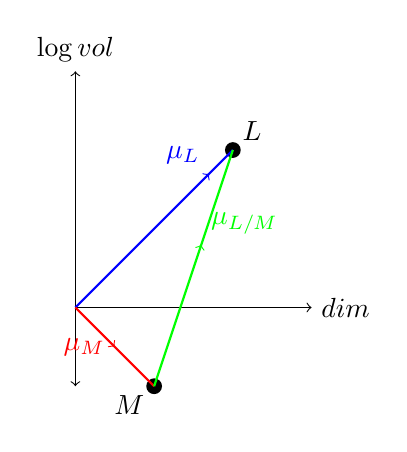
\begin{tikzpicture}
        % Draw axes
        \draw[->] (0,0) -- (3,0) node[right] {$dim$};
        \draw[->] (0,0) -- (0,3) node[above] {$\log vol$};
        \draw[->] (0,0) -- (0,-1);
        % Plot points L and M
        \fill (2,2) circle (0.1) node[above right] {$L$};
        \fill (1,-1) circle (0.1) node[below left] {$M$};

        % Draw lines from origin to L and M with colors
        \draw[thick, blue] (0,0) -- (2,2);
        \draw[thick, red] (0,0) -- (1,-1);

        % Draw line between M and L with color
        \draw[thick, green] (1,-1) -- (2,2);

        % Add mu annotations with matching colors
        \draw[->, blue] (1.5,1.5) -- (1.7,1.7) node[above left] {$\mu_L$};
        \draw[->, red] (0.3,-0.3) -- (0.5,-0.5) node[left] {$\mu_M$};
        \draw[->, green] (1.5,0.5) -- (1.6,0.8) node[above right] {$\mu_{L/M}$};
    \end{tikzpicture}
    \caption{Geometric meaning of slope in canonical plot}
\end{figure}
Given two sublattices $M_1,M_2 \subset L$, if we apply lemma \ref{volume-of-lattice} to the sublattices
$M_1/M_1\cap M_2$ and $M_2/M_1\cap M_2$ in $M_1+M_2/M_1\cap M_2$, we get
\[\vol(M_1/M_1 \cap M_2)\vol(M_2/M_1\cap M_2) \ge \vol(M_1+M_2/M_1\cap M_2)\]
or equivalently
\begin{prop}\label{parallelogram-rule}\cite[Proposition 4.3]{MR2127941}
    Suppose $M_1,M_2$ are sublattices of $L$ then
    \[\log\vol(M_1)+\log\vol(M_2) \ge \log\vol(M_1+M_2)+\log\vol(M_1\cap M_2)\]
\end{prop}


Grayson called this the parallelogram rule, as the geometric meaning of  proposition \ref{parallelogram-rule} is
illustrated in the figure \ref{Grason's parallelogram rule}.
\begin{figure}[hbt!]
    \centering
    \begin{tikzpicture}
        % Coordinates
        \coordinate (A) at (0,0);
        \coordinate (B) at (4,2);
        \coordinate (C) at (6,0);
        \coordinate (D) at (2,-2);
        \coordinate (F) at (4,2.5);
        % Drawing the parallelogram
        \draw (A) -- (B) -- (C) -- (D) -- cycle;

        % Labels
        \node at (A) [above left] {$M_1 \cap M_2$};
        \node at (F) [above] {$M_1$};
        \node at (C) [above right] {$M_1 + M_2$};
        \node at (D) [below] {$M_2$};

        % Points
        \fill[cyan] (A) circle (2pt);
        \fill[cyan] (B) circle (2pt);
        \fill[cyan] (C) circle (2pt);
        \fill[cyan] (D) circle (2pt);
        \fill[cyan] (F) circle (2pt);
    \end{tikzpicture}
    \caption{{Grason's parallelogram  rule}}
    \label{Grason's parallelogram  rule}
\end{figure}
The \textbf{vertices} of the profile are the extremal/lowest points of the plot. Clearly the two points
$(0,0)$ and $(n,\log\vol(L))$ are vertices of the plot of the lattices $L$ with $\rk(L)=n$. The following lemma states the situation for other vertices
of the profile
\begin{lemma}\label{upper-ver}\cite[Lemma 4.4]{MR2127941}
    Suppose that $M_\ast$ is a lattice with with the point $\ell(M_\ast)$ as a vertex of the profile. If $M$ is any other sublattice such that
    $\ell(M)$ is also a vertex of the profile, then we must have either $M \subset M_\ast$ or $M_\ast \subset M$.
\end{lemma}
\begin{figure}[H]
    \centering
    \begin{tikzpicture}
        % Coordinates
        \coordinate (A) at (0,0);
        \coordinate (B) at (4,2);
        \coordinate (C) at (6,0);
        \coordinate (D) at (2,-2);
        \coordinate (F) at (4,2.5);
        \coordinate (E) at (5,-1.5);
        \coordinate (G) at (-1,0);
        \coordinate (H) at (8,-0.5);

        % Drawing the parallelogram
        \draw (A) -- (B) -- (C) -- (D) -- cycle;

        % Labels
        \node at (A) [above left] {$M \cap M_*$};
        \node at (F) [above] {$M$};
        \node at (C) [above right] {$M + M_*$};
        \node at (D) [below] {$M_*$};
        % Points
        \fill[cyan] (A) circle (2pt);
        \fill[cyan] (B) circle (2pt);
        \fill[cyan] (C) circle (2pt);
        \fill[cyan] (D) circle (2pt);
        \fill[cyan] (F) circle (2pt);
        \fill[cyan] (E) circle (2pt);

        % draw additional lines
        \draw[gray] (G) -- (D)-- (E) -- (H);
    \end{tikzpicture}
    \caption{Illustration for lemma \ref{upper-ver}}
    \label{figure33}
\end{figure}
\begin{proof}
    We refer to figure \ref{figure33}. Clearly we can see that the point $\ell(M\cap M_*$) lies somewhere on the left of both
    $\ell(M)$ and $\ell(M_*)$. Similarly, the point $\ell(M+M_*)$ lies somewhere inclusively to the right of $\ell(M)$ and $\ell(M_*)$.
        By the paralellogram rule, the point $ell(M)$ will therefore be above the boundary points
    $\ell(M\cap M_*)$, $\ell(M_*)$ and $\ell(M+M_*)$. If $M$ is also a vertex of the profile, the parallelogram must degenerate. In particular we either have
    $M \cap M*=M$, in which $M\subset M_*$, or $M+M_* = M$, in which $M_* \subset M$.
\end{proof}
An immediate consequence is that
\begin{theorem}\label{filtration}\cite[Theorem 1.18]{MR780079}
    The vertices of the profile of a lattice $L$ are represented by unique sublattices, and they form a chain.
\end{theorem}
For a given lattice $L$, we call the chain of sublattices in theorem \ref{filtration} the \textbf{canonical filtration} of $L$. Assume that the canonical filtration for $L$
is
\[\mathcal{F}: 0 = L_0 \subset L_1 \subset L_2 \subset \cdots \subset L_{k-1} \subset L_k = L \]
then it can be seen from the diagram that
\begin{enumerate}
    \item $L_i/L_{i-1}$ is semi-stable for all $1 \le i \le k$, as the profile of $L_i/L_{i-1}$  is just a straight line segment connecting $\ell(L_{i-1})$ to $\ell(L_i)$.
    \item $\mu(L_i/L_{i-1}) \le \mu(L_{i+1}/L_i)$ for all $1 \le i \le k-1$.
\end{enumerate}
These two conditions is also sufficent for a chain to be a canonical filtration
\begin{theorem}\label{Grayson's criterion}\cite[Corollary 1.30]{MR780079}
    Suppose
    \[\mathcal{F}: 0 = L_0 \subset L_1 \subset L_2 \subset \cdots \subset L_{k-1} \subset L_k = L \]
    is a chain of lattices such that $L_i/L_{i-1}$ is semi-stable and the slope $L_i/L_{i-1}$ is not larger than the slope of $L_{i+1}/L_i$.
    Then this chain is the canonical filtration.
\end{theorem}
\begin{figure}[ht]
    \centering
    \begin{tikzpicture}
        % Coordinates
        \coordinate (A) at (0,0);
        \coordinate (B) at (4,2);
        \coordinate (C) at (6,0);
        \coordinate (D) at (2,-2);
        \coordinate (F) at (4,2.5);
        \coordinate (E) at (5,-1.5);
        \coordinate (G) at (-1,0);
        \coordinate (H) at (8,-0.5);

        % Drawing the parallelogram
        \draw (A) -- (B) -- (C) -- (D) -- cycle;

        % Labels
        \node at (A) [above left] {$M \cap L_{i-1}$};
        \node at (F) [above] {$M$};
        \node at (C) [above right] {$M + L_{i-1}$};
        \node at (D) [below] {$L_{i-1}$};
        \node at (E) [below] {$L_i$};

        % Points
        \fill[cyan] (A) circle (2pt);
        \fill[cyan] (B) circle (2pt);
        \fill[cyan] (C) circle (2pt);
        \fill[cyan] (D) circle (2pt);
        \fill[cyan] (F) circle (2pt);
        \fill[cyan] (E) circle (2pt);

        % draw additional lines
        \draw[gray] (G) -- (D)-- (E) -- (H);
    \end{tikzpicture}
    \caption{Canonical filtration}
    \label{figure34}
\end{figure}
\begin{proof}
    Suppose $M$ to be any other sublattice of $L$. We want to know that $\ell(M)$ lies
    above the plot $P$ of the $\ell(L_i)$. We prove this by induction on the index $i$ such that if $M \subset L_i$
    \begin{itemize}
        \item If $i=1$ then $M\subset L_1$. Since $L_1 $ is semi-stable, we must have $\ell(M)$ lies above the line connecting $(0,0)$ and $\ell(L_1)$. Hence $\ell(M)$ lies above the plot $P$.
        \item Suppose that $M\subset L_i$ for $i>1$. Then $M+L_{i-1} \subset L_i$ contains $L_{i-1}$. Therefore, it corresponds to the point lies above the line connecting $\ell(L_{i-1})$ and $\ell(L_i)$, thus lies above $P$.         By induction, the fact that $(M\cap L_{i-1}) \subset L_{i-1}$ implies $\ell(M\cap L_{i-1})$ lies above the plot $P$. Using the parallelogram rule, the point $\ell(M)$ must then also lie above the plot $P$.
    \end{itemize}
    Thus any chain satisfies the conditions given in the theorem is a canonical filtration.
\end{proof}
\section{$\rho$ semi-stability}
\subsection{$\rho$-definition}
We are now ready to define the $\rho$-definition of semi-stable lattice. Recall that
we define the space of lattices of rank $n$ by $X_n := K \backslash \text{GL}_n(\mathbb{R})$, where $K$ is the orthogonal subgroup
\begin{definition}[\label  = $\rho$-definition]\label{ss2}
    Let $x \in X_n$ be an arbitrary lattice, then the lattice $x$ is called \textbf{$\rho$-semi-stable} if and only if its degree of instability $\deg_{\text{inst}}(x)\ge 0$, where
    \[\deg_{\text{inst}}(x):= \min_{Q \in ParSt, \gamma \in \text{GL}(\mathbb{Q})/Q_i(\mathbb{Q})}\left\langle \rho_Q, H_Q(x\gamma) \right\rangle\]
    and $\text{ParSt}$ stands for the set of standard parabolic subgroup of $\GLn$ as defined in definition \ref{parst}.
\end{definition}
\subsection{Some basic properties}
We first have an elementary lemma and refer to the references for the proof.
\begin{lemma}\label{ss-equiv}\citetext{\citealp[Lemma 2.2.1]{MR3969872}; \citealp[Proposition 4.2.3]{patnaik2025borel}}

    Given $x \in X_n$, then the following are equivalent
    \begin{enumerate}
        \item $\deg_{\text{inst}}(x) \ge 0$.
        \item For every standard parabolic subgroup $P\subset G$ and $\omega \in \widehat{\Delta}_P$ we have \[\left\langle \omega,H_P(x\delta)\right\rangle \ge 0\] for each $\delta \in G(\mathbb{Q})/P(\mathbb{Q})$.
        \item For every maximal parabolic subgroup $Q\subset G$ and $\omega \in \widehat{\Delta}_Q$ we have \[\left\langle \omega,H_Q(x\delta)\right\rangle \ge 0\] for each $\delta \in G(\mathbb{Q})/Q(\mathbb{Q})$.
    \end{enumerate}
\end{lemma}
\subsection{Check for semi-stability}\label{semi-stable-verified}
From lemma \ref{ss-equiv}, to check whether $x \in G$ is semi-stable, we just need to verify whether $$\left\langle \omega,H_Q(x\delta)\right\rangle \ge 0.$$
for $\omega \in \widehat{\Delta}_Q$ and $Q \subset G$ a standard maximal parabolic subgroup.
From lemma \ref{coeff-H(J)}
\[H_B = H_Q+H(Q)_{\ast B}\]
where $H_Q$ is a scalar multiple of $\lambda_i^\vee$ for $Q = Q_i$ and $H(Q)_{\ast B}$ is a linear combination of $\alpha_j^\vee$ for $ j \ne i$.
On the other hand, since $Q$ is a maximal standard parabolic subgroup of $G$,
$\omega$ is proportional to $\lambda_i.$ Thus $$\left\langle \omega H(Q)_{\ast B}(x\gamma)\right\rangle =0.$$ In particular, we can replace $H_Q$ by $H_B$ in verifying semi-stability.
Write
\[ x\gamma = kan, \quad k \in K, a \in A, n \in N,\]
as in Iwasawa decomposition, and set $H_B(x) = H$ where $H = \exp(a)$. In particular, if
\[a = \begin{bmatrix}
        a_1    & 0      & \ldots & 0      \\
        0      & a_2    & \ldots & 0      \\
        \vdots & \vdots & \vdots & \vdots \\
        0      & 0      & \ldots & a_n
    \end{bmatrix}\]
then
\begin{equation}
    \left\langle \rho_{Q_i}, H_B(x\gamma) \right\rangle = \dfrac{n}{2}\log(a_1a_2\ldots a_i) \label{volume - H_P}
\end{equation}
Thus, to check for the semi-stability of a lattice $x$, we just need to look at the
$A$-coordinate of $x\gamma$ for every $\gamma \in G(\mathbb{Q})/Q_i(\mathbb{Q})$, and verify whether the following system holds
\begin{align*}
    \begin{cases}
        a_1 \ge 1   \\
        a_1a_2\ge 1 \\
        \ldots      \\
        a_1a_2\ldots a_n \ge 1
    \end{cases}
\end{align*}
\section{Canonical pair}
Consider a pair $(P,\delta)$ of a standard parabolic subgroup $P \subsetneq G$ and $\delta \in G(\mathbb{Q})/P(\mathbb{Q})$. Such a pair is called \textbf{destabilizing} for $x$ if
\[\left\langle \rho_P, H_P(x\delta)\right\rangle = \deg_{\text{inst}}(x)\]
Such a pair is called \textbf{extremal} for $x$ if for any standard parabolic $Q \subset P$ such that
\[\left\langle \rho_Q, H_Q(x\delta)\right\rangle = \left\langle \rho_P, H_P(x\delta)\right\rangle\]
then $Q=P$.
\begin{definition}
    A pair $(P,\delta)$ that is both \textit{destabilizing} and \textit{extremal} for $x$ is called a \textbf{canonical pair} for $x$.
\end{definition}
A canonical pair for $x$, if exists, will be denoted by $\cpx:=(P,\delta)$. A priori, it is not clear whether $\cpx$ exists or not.
We will show that it is in fact equivalent to the notion of canonical filtration introduced in the previous sections, and deduce that
$\cpx$ must exist and it is unique.

We obtain the following lemma as a consequence of the definition of canonical pair
\begin{lemma}\label{canonical-pair}\citetext{\citealp[Lemma 2.3.2]{MR3969872}; \citealp[Lemma 4.2.5]{patnaik2025borel}}
    Let $x \in X_n$  and $(P,\delta)$ be a pair with $P \subsetneq G$ be standard parabolic subgroup and
    $\delta \in G(\mathbb{Q})/P(\mathbb{Q})$. Then
    \begin{enumerate}
        \item If $(P,\delta)$ is destabilizing for $x$, then $\deg_{inst}^P(x\delta) \ge 0$. \label{destabilizing}
        \item If $(P,\delta) $ is extremal for $x$, then $\left\langle \alpha, H_P(x\delta)\right\rangle < 0$ for any $\alpha \in \Delta_P$.\label{extremal}
    \end{enumerate}
\end{lemma}
\begin{proof}
    For the first part, let $Q \subset P$ be any standard parabolic, then
    \[\rho_Q = \rho_P + \rho_Q^P\]
    Thus, for any $\eta \in P(\mathbb{Q})/Q(\mathbb{Q})$
    \begin{align*}
        \left\langle \rho_Q^P,H_Q(x\gamma\eta)\right\rangle & = \left\langle\rho_Q,H_Q(x\gamma\eta)\right\rangle - \left\langle\rho_P,H_P(x\gamma\eta)\right\rangle \\                                                 & = \left\langle\rho_Q,H_Q(x\gamma\eta)\right\rangle -\deg_{inst}(x) \ge 0
    \end{align*}
    For the second part, we can pick a standard parabolic $Q \subset G$ containing $P$ such that $P$ is maximal in $Q$. In particular, we have
    $\Delta^{Q}_P = \{\alpha\}$. Then
    \begin{align*}
        \left\langle\rho_P^Q,H_P(x\delta)\right\rangle & = \left\langle\rho_P,H_P(x\gamma)\right\rangle - \left\langle\rho_Q,H_Q(x\gamma\eta)\right\rangle \\
                                                       & = \deg_{inst}(x) - \left\langle\rho_Q,H_Q(x\gamma\eta)\right\rangle <0
    \end{align*}
    Since $\rho_P^Q$ and $\alpha$ are proportional by a positive number, the result follows immediately.\end{proof}
